\documentclass{beamer}

\usepackage[utf8]{inputenc}
 
\usepackage{listings}
\usepackage{color}
%
%\usepackage{graphicx}
%\graphicspath{ {./} }
%
\usepackage[T1]{fontenc}
\usepackage{libertine}
\usepackage[scaled=0.6]{beramono}
\usepackage[export]{adjustbox}

\lstset{
  basicstyle=\linespread{0.65}\ttfamily\small,
  breakatwhitespace=false,     
  breaklines=true,         
  captionpos=b,          
  keepspaces=true,         
  showspaces=false,        
  showstringspaces=false,
  showtabs=false,          
  tabsize=2,
  emph={  
    OneToMany, OneShot, ManyToOne
  },
  emphstyle={\color{orange}\bfseries}
}

\lstdefinelanguage{logic}{
  morekeywords={
    datatype,
    type,
    fun,
    val,
    predicate,
    where, only,
    if, then, else,
    and, or, not,
    lemma,
    theorem,
    of,
    have,
    assume, case, apply, done, by, proof, qed,
    goal
  },
  mathescape
}

\lstdefinelanguage{normal_lang}{
  morekeywords={
    bind, rslt, fun, app, unt, pair,
    mkChn, sync, fst, snd, lft, rht,
    spawn, case, of, sendEvt, recvEvt
  }
}

\lstdefinelanguage{sugar_lang}{
  morekeywords={
    datatype,
    type,
    fun,
    val,
    predicate,
    only, if, then, else,
    and, or, not,
    lemma,
    theorem,
    of,
    fun,
    bind, rslt, unt, pair,
    chn, lft, rht,
    sendEvt, recvEvt
  }
}

\title{A Mechanized Theory of Communication Analysis in CML}

%\usetheme{lucid}
\begin{document}

\begin{frame}
  \titlepage
\end{frame}

\begin{frame}
\frametitle{Concurrent ML}
\begin{itemize}
\item extension of Standard ML
\item concurrency and synchronization
\item synchronized communication over channels: send event, receive event
\item composition of events: choose event, wrap event ...
\end{itemize}
\end{frame}

\begin{frame}[fragile]
\frametitle{Concurrent ML}
\begin{lstlisting}[language=ML]

type thread_id
val spawn : (unit -> unit) -> thread_id

type 'a chan
val channel : unit -> 'a chan

type 'a event
val sync: 'a event -> 'a

val recvEvt: 'a chan -> 'a event
val sendEvt: 'a channel * 'a -> unit event

val send: 'a chan * 'a -> unit
fun send (ch, v) = sync (sendEvt (ch, v))

val recv: 'a chan -> 'a
fun recv ch = sync (recvEvt ch)

\end{lstlisting}
\end{frame}


\begin{frame}[fragile]
	\frametitle{Concurrent ML}
\begin{columns}
\begin{column}{0.5\textwidth}
\begin{lstlisting}[language=ML, mathescape]
structure Serv : SERV =
struct 
  datatype serv =
    S of (int * int chan) chan

  fun make () =
  let 
    val reqCh = channel ()
    fun loop state =
    let
      val (v, replCh) = recv reqCh
      val () = send (replCh, state)
    in
      loop v
    end
    val () = spawn (fn () => loop 0)
  in
    S reqCh
  end 
\end{lstlisting}
\end{column}


\begin{column}{0.5\textwidth}
\begin{lstlisting}[language=ML, mathescape]
  fun call (server, v) =
  let 
    val S reqCh = server
    val replCh = channel () 
    val () = send (reqCh, (v, replCh))
  in
    recv replCh
  end
end

signature SERV =
sig 
  type serv
  val make : unit -> serv
  val call : serv * int -> int
end
\end{lstlisting}
\end{column}
\end{columns}
\end{frame}



\begin{frame}
\frametitle{Isabelle/HOL}
\begin{itemize}
\item interactive theorem proving assistant; proof assistant
\item trusted kernel of manipulation rules
\item unification and rewriting
\item simply typed terms
\item propositions as boolean typed terms
\item higher order terms
\item inductive data
\item computable recursive functions
\item inductive predicates
\item inductive reasoning
\item tactics and composition
\end{itemize}
\end{frame}



\begin{frame}[fragile]
	\frametitle{Isabelle/HOL}
\begin{columns}
\begin{column}{0.5\textwidth}
\begin{lstlisting}[language=logic, mathescape]
$\vdash$ P1 $\vee$ P2 $\rightarrow$ Q
proof
  assume P1 $\vee$ P2:
    case P1:
      have $\vdash$ P1 $\rightarrow$ Q by A
      have $\vdash$ Q by modus ponens
    case P2:
      have $\vdash$ P2 $\rightarrow$ Q by B    
      have $\vdash$ Q by modus ponens
    have P1 $\vdash$ Q, P2 $\vdash$ Q
    have $\vdash$ Q by disjunction elimination
  have P1 $\vee$ P2 $\vdash$ Q
  have $\vdash$ P1 $\vee$ P2 $\rightarrow$ Q
    by implication introduction  
qed
\end{lstlisting}
\end{column}

\begin{column}{0.5\textwidth}
\begin{lstlisting}[language=logic, mathescape]
$\vdash$ P1 $\vee$ P2 $\rightarrow$ Q
apply (rule impI)
  P1 $\vee$ P2 $\vdash$ Q
apply (erule disjE)
  P1 $\vdash$ Q
* P2 $\vdash$ Q
apply (insert A)
  P1, P1 $\rightarrow$ Q $\vdash$ Q
* P2 $\vdash$ Q
apply (erule mp)
  P1 $\vdash$ P1
* P2 $\vdash$ Q
apply assumption 
  P2 $\vdash$ Q
apply (insert B)
  P2, P2 $\rightarrow$ Q $\vdash$ Q
apply (erule mp)
  P2 $\vdash$ P2
apply assumption 
done
\end{lstlisting}
\end{column}
\end{columns}
\end{frame}


\begin{frame}
\frametitle{Analysis}
\begin{itemize}
\item communication classification: one-shot, one-to-many, many-to-one, many-to-many
\item control flow analysis
\item channel liveness
\item algorithm vs constraints
\item structural recursion vs fixpoint accumulation
\item performance improvements
\item safety
\end{itemize}
\end{frame}



\begin{frame}[fragile]
\frametitle{Communication Classification}
\begin{columns}
\begin{column}{0.5\textwidth}
\begin{lstlisting}[language=ML, mathescape]
structure Serv : SERV =
struct 

  datatype serv =
    S of (int * int chan) chan 

  fun make () =
  let 
    val reqCh = ManyToOne.channel ()
    fun loop state =
    let
      val (v, replCh) = ManyToOne.recv reqCh
      val () = OneShot.send (replCh, state)
    in
      loop v
    end
    val () = spawn (fn () => loop 0)
  in
    S reqCh
  end 
\end{lstlisting}
\end{column}


\begin{column}{0.5\textwidth}
\begin{lstlisting}[language=ML, mathescape]
  fun call (server, v) =
  let 
    val S reqCh = server
    val replCh = OneShot.channel ()
    val () = ManyToOne.send (reqCh, (v, replCh))
  in
    OneShot.recv replCh
  end

end

val server = Serv.make ()

val () =
  spawn (fn () => Serv.call (server, 35));
  (spawn fn () => 
    Serv.call (server, 12); 
    Serv.call (server, 13)
  );
  spawn (fn () => Serv.call (server, 81));
  spawn (fn () => Serv.call (server, 44))
\end{lstlisting}
\end{column}
\end{columns}
\end{frame}


\begin{frame}
\frametitle{Synchronization}
\begin{itemize}
\item uniprocessor; dispatch scheduling
\item multiprocessor; mutex and compare-and-swap
\item synchronization state
\item sender and receiver thread containers
\item message containers
\end{itemize}
\end{frame}

\begin{frame}[fragile]
	\frametitle{Formal Mechanized Theory}
\begin{itemize}
\item Isabelle/HOL  
\item $\sim$ 1421 lines of definitions  
\item $\sim$ 3052 lines of completed proofs 
\item syntax-directed rules
\end{itemize}
\end{frame}



\begin{frame}[fragile]
	\frametitle{Syntax}
\begin{lstlisting}[language=logic, mathescape]
datatype name = Nm string

datatype term = 
  Bind name complex term 
| Rslt name

and complex = 
  Unt
| MkChn
| Atom atom
| Spwn term 
| Sync name
| Fst name
| Snd name
| Case name name term name term 
| App name name

and atom = 
  SendEvt name name
| RecvEvt name
| Pair name name
| Lft name
| Rht name
| Fun name name term 
\end{lstlisting}
\end{frame}


\begin{frame}[fragile]
	\frametitle{Syntax}
\begin{columns}
\begin{column}{0.5\textwidth}
\begin{lstlisting}[language=normal_lang, mathescape]
bind u1 = unt
bind r1 = rht u1
bind l1 = lft r1
bind l2 = lft l1

bind mksr = fun _ x2 => 
(
  bind k1 = mkChn
  bind srv = fun srv' x3 =>
  (
    bind e1 = recvEvt k1
    bind p1 = sync e1
    bind v1 = fst p1
    bind k2 = snd p1 
    bind e2 = sendEvt k2 x3
    bind z5 = sync e2
    bind z6 = app srv' v1
    rslt z6 
  )
  bind z7 = spawn
  (
    bind z8 = app srv r1
    rslt z8 
  )
  rslt k1
)
\end{lstlisting}
\end{column}

\begin{column}{0.5\textwidth}
\begin{lstlisting}[language=normal_lang, mathescape]
bind rqst = fun _ x4 =>
(
  bind k3 = fst x4
  bind v2 = snd x4
  bind k4 = mkChn
  bind p2 = pair v2 k4
  bind e3 = sendEvt k3 p2
  bind z9 = sync e3
  bind e4 = recvEvt k4
  bind v3 = sync e4
  rslt v3
)

bind srvr = mksr u1
bind z10 = spawn
( 
  bind p3 = pair srvr l1
  bind z11 = app rqst p3
  rslt z11
)
bind p4 = pair srvr l2
bind z12 = app rqst p4
rslt z12
\end{lstlisting}
\end{column}
\end{columns}
\end{frame}

\begin{frame}[fragile]
\frametitle{Dynamic Semantics}
\begin{lstlisting}[language=logic, mathescape]
datatype dynamic_step =
  DSeq name
| DSpwn name
| DCll name
| DRtn name 

type dynamic_path = dynamic_step list

datatype chan =
  Chan dynamic_path name 

datatype dynamic_value = 
  VUnt
| VChn chan
| VAtm atom (name -> dynamic_value option)

type environment =
  name -> dynamic_value option
\end{lstlisting}
\end{frame}

\begin{frame}[fragile]
\frametitle{Dynamic Semantics}
\begin{lstlisting}[language=logic, mathescape]
predicate seqEval: complex -> environment -> dynamic_value -> bool 

predicate callEval: complex -> env -> term -> env -> bool 

datatype contin = Ctn name tm env

type stack = contin list

datatype state = Stt program env stack 

type pool = dynamic_path -> state option

predicate leaf: pool -> dynamic_path -> bool

type corresp = dynamic_path * chan * dynamic_path

type communication = corresp set 

predicate dynamicEval: pool -> communication -> pool -> communication -> bool

predicate star: ('a -> 'a -> bool) -> 'a -> 'a -> bool 
\end{lstlisting}
\end{frame}


\begin{frame}[fragile]
	\frametitle{Dynamic Communication}
\begin{lstlisting}[language=logic, mathescape]
predicate isSendPath: pool -> chan -> dynamic_path -> bool 

predicate isRecvPath: pool -> chan -> dynamic_path -> bool

predicate forEveryTwo: ('a -> bool) -> ('a -> 'a -> bool) -> bool

predicate ordered: 'a list -> 'a list -> bool

predicate oneToMany: tm -> chan -> bool

predicate manyToOne: tm -> chan -> bool

predicate oneToOne: tm -> chan -> bool

predicate oneShot: tm -> chan -> bool

predicate oneSync: tm -> chan -> bool
\end{lstlisting}
\end{frame}

\begin{frame}[fragile]
	\frametitle{Dynamic Communication}
\begin{lstlisting}[language=logic, mathescape]
predicate oneToMany: tm -> chan -> bool where
  intro: t$_0$ chan .
    star dynamicEval [[] -> (Stt t$_0$ [->] [])] {} pool comm,
    forEveryTwo (isSendPath pool chan) ordered
  $\vdash$ oneToMany pool chan
\end{lstlisting}
\end{frame}


\begin{frame}[fragile]
	\frametitle{Static Semantics}
\begin{lstlisting}[language=logic, mathescape]
datatype static_value =
  SUnt
| SChn name
| SAtm atom 

type static_value_map =
  name -> static_value set

fun resultName: term -> name

predicate staticEval: static_value_map -> static_value_map -> term -> bool
\end{lstlisting}
\end{frame}

\begin{frame}[fragile]
	\frametitle{Static Semantics}
\begin{columns}
\begin{column}{0.5\textwidth}
\begin{lstlisting}[language=sugar_lang, mathescape]
val staticEnv: name -> static_value set =
(
  u1 -> {unt},
  r1 -> {rht u1},
  l1 -> {lft r1},
  l2 -> {lft l1},
  mksr -> {fun  _ x2 => ...},
  x2 -> {unt},
  k1 -> {chn k1},
  srv -> {fun srv' x3 => ...},
  srv' -> {fun srv' x3 => ...},
  x3 -> {rht u1, lft r1, lft l1},
  e1 -> {recvEvt k1},
  p1 -> {pair v2 k4},
  v1 -> {lft r1, lft l1},
  k2 -> {chn k4},
  e2 -> {sendEvt k2 x3},
  z5 -> {unt},
  z7 -> {unt},
  u5 -> {unt},
  rqst -> {fun _ x4 => ...},
\end{lstlisting}
\end{column}

\begin{column}{0.5\textwidth}
\begin{lstlisting}[language=sugar_lang, mathescape]
  x4 -> {pair srvr l1, pair srvr l2},
  k3 -> {chn k1},
  v2 -> {lft r1, lft l1},
  k4 -> {chn k4},
  p2 -> {pair v2 k4},
  e3 -> {sendEvt k3 p2},
  z9 -> {unt},
  e4 -> {recvEvt k4},
  v3 -> {rht u1, lft r1, lft r2},
  srvr -> {chn k1},
  z10 -> {unt},
  p3 -> {pair srvr l1},
  z11 -> {rht u1, lft r2},
  p4 -> {pair srvr l2},
  z12 -> {rht u1, lft l1}
)

val staticComm: name -> static_value set =
(
  k1 -> {pair v2 k4},
  k4 -> {rht u1, lft l1, lft l2}
)
\end{lstlisting}
\end{column}
\end{columns}
\end{frame}


\begin{frame}[fragile]
	\frametitle{Static Communication}
\begin{lstlisting}[language=logic, mathescape]
predicate staticFlowsAccept: static_value_map -> graph -> term -> bool

predicate staticTraceable:
  flow set -> tm_id -> (tm_id -> bool) -> static_path -> bool

predicate staticInclusive: static_path -> static_path -> bool

predicate uncompetitive: static_path -> static_path -> bool

predicate staticOneToMany: term -> name -> bool

predicate staticManyToOne: term -> name -> bool

predicate staticOneToOne: term -> name -> bool

predicate staticOneShot: term -> name -> bool

predicate staticOneSync: term -> name -> bool
\end{lstlisting}
\end{frame}

\begin{frame}[fragile]
	\frametitle{Static Communication}
\begin{lstlisting}[language=logic, mathescape]
predicate staticOneToMany: term -> name -> bool where
  intro: staticEnv staticComm t graph n$_c$ .
    staticEval staticEnv staticComm t,
    staticFlowsAccept staticEnv graph t,
    forEveryTwo (staticTraceable graph (termId t)
      (staticSendId staticEnv t n$_c$)) uncompetitive
  $\vdash$ staticOneToMany t n$_c$
\end{lstlisting}
\end{frame}


\begin{frame}
\frametitle{Soundness}
\begin{itemize}
\item induction on transition system 
\item generalization to intermediate semantic data structures 
\item skewing of induction direction
\item reversing of inference direction  
\item preservation
\end{itemize}
\end{frame}


\begin{frame}[fragile]
	\frametitle{Soundness}
\begin{lstlisting}[language=logic, mathescape]
theorem staticOneToManySound: t$_0$ n$_c$ path$_c$ . 
  staticOneToMany t$_0$ n$_c$
$\vdash$ oneToMany t$_0$ (Chan path$_c$ n$_c$)

theorem staticManyToOneSound: t$_0$ n$_c$ path$_c$ . 
  staticManyToOne t$_0$ n$_c$
$\vdash$ manyToOne t$_0$ (Chan path$_c$ n$_c$)

theorem staticOneToOneSound: t$_0$ n$_c$ path$_c$ . 
  staticOneToOne staticEnv t$_0$ n$_c$
$\vdash$ oneToOne t$_0$ (Chan path$_c$ n$_c$)

theorem staticOneShotSound: t$_0$ n$_c$ path$_c$ .
  staticOneShot t$_0$ n$_c$
$\vdash$ oneShot t$_0$ (Chan path$_c$ n$_c$)

theorem staticOneShotSound: t$_0$ n$_c$ path$_c$ .
  staticOneSync t$_0$ n$_c$
$\vdash$ oneSync t$_0$ (Chan path$_c$ n$_c$)
\end{lstlisting}
\end{frame}


\begin{frame}[fragile]
	\frametitle{Soundness}
\begin{lstlisting}[language=logic, mathescape]
lemma staticEvalSound: t$_0$ pool comm staticEnv staticComm path t env stack n v .
  staticEval staticEnv staticComm t$_0$, 
  star dynamicEval [[] -> (Stt t$_0$ [->] [])] {} pool comm,
  pool path = Some (Stt t env stack), 
  env n = Some v
$\vdash$ abstract v $\in$ staticEnv n 
\end{lstlisting}
\end{frame}


\begin{frame}
\frametitle{Higher Precision Analysis}
\begin{itemize}
\item different channel instances with same name  
\item channel liveness analysis
\item trimmed graph
\item paths from channel creation site
\item paths along sending transitions 
\end{itemize}
\end{frame}

\begin{frame}[fragile]
\frametitle{Higher Precision Analysis}
\begin{lstlisting}[language=logic, mathescape]
predicate staticChanLive:
  static_value_map -> tm_id_map -> tm_id_map -> name -> term -> bool

predicate staticPathLive:
  graph -> tm_id_map -> tm_id_map -> tm_id -> (tm_id -> bool) -> static_path -> bool
\end{lstlisting}
\end{frame}

\begin{frame}
\frametitle{Higher Precision Analysis}
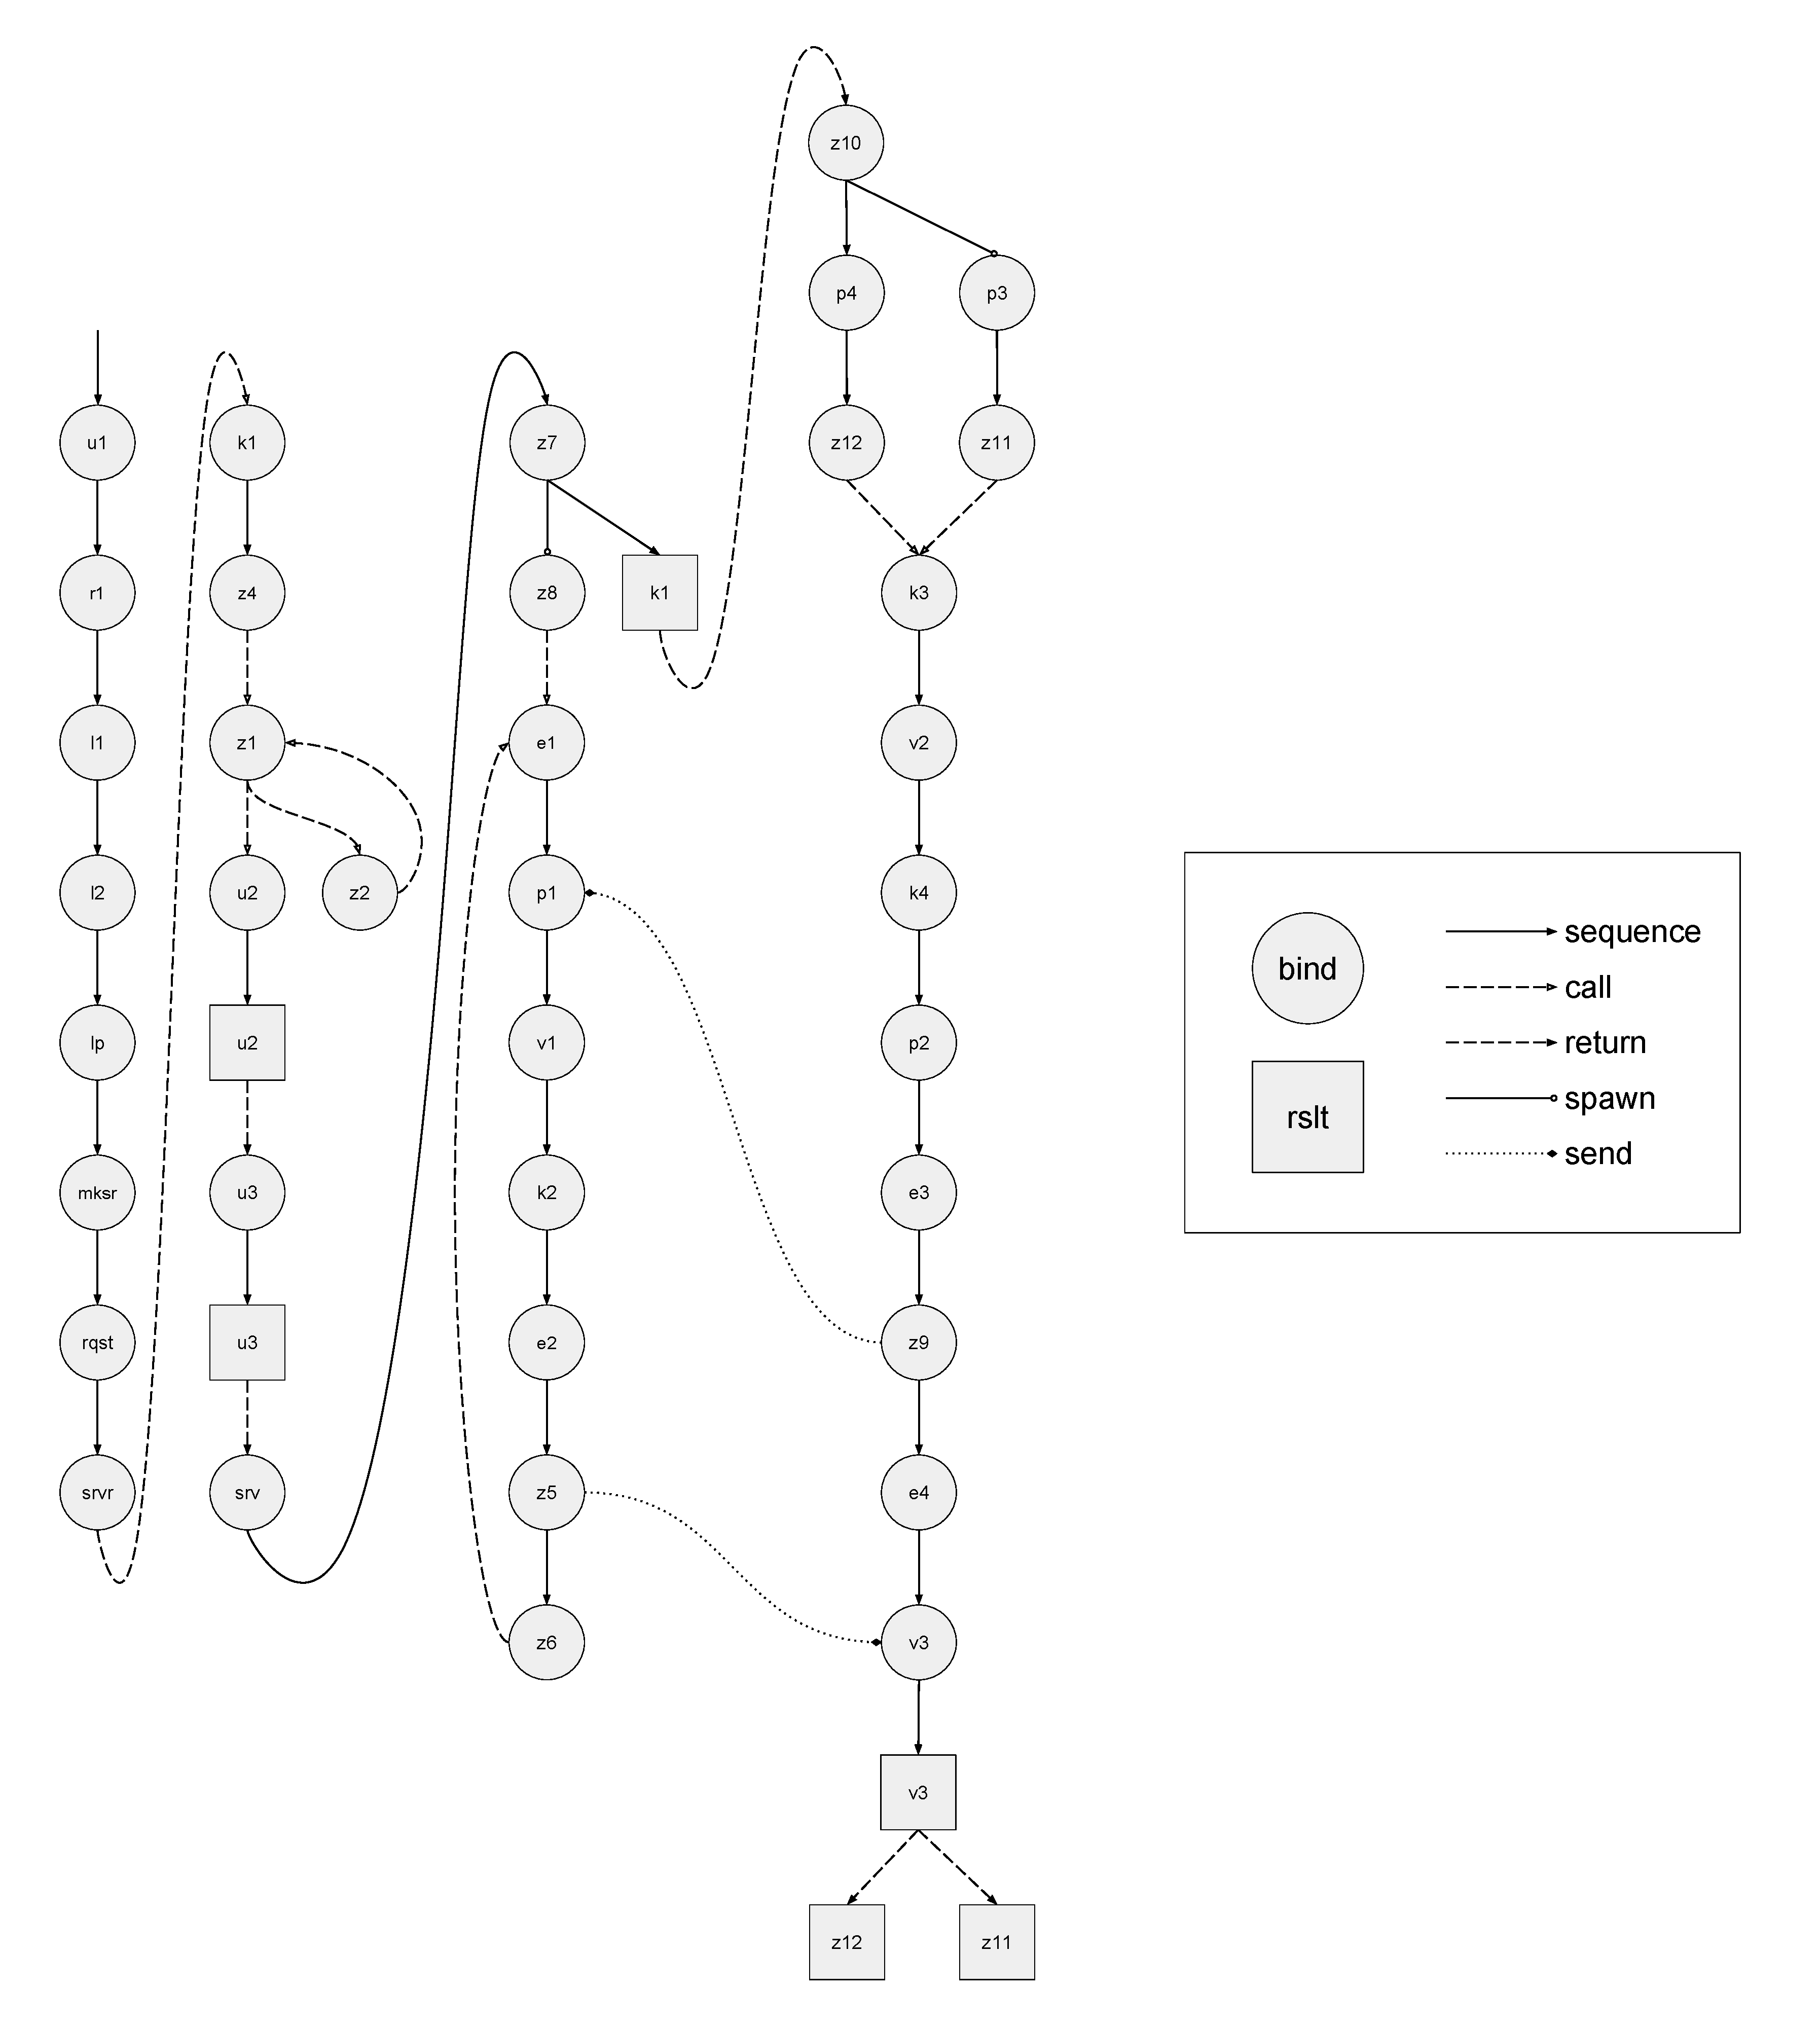
\includegraphics[width=.7\textwidth]{cml-graph-lp.pdf}
\end{frame}

\begin{frame}
\frametitle{Higher Precision Analysis}
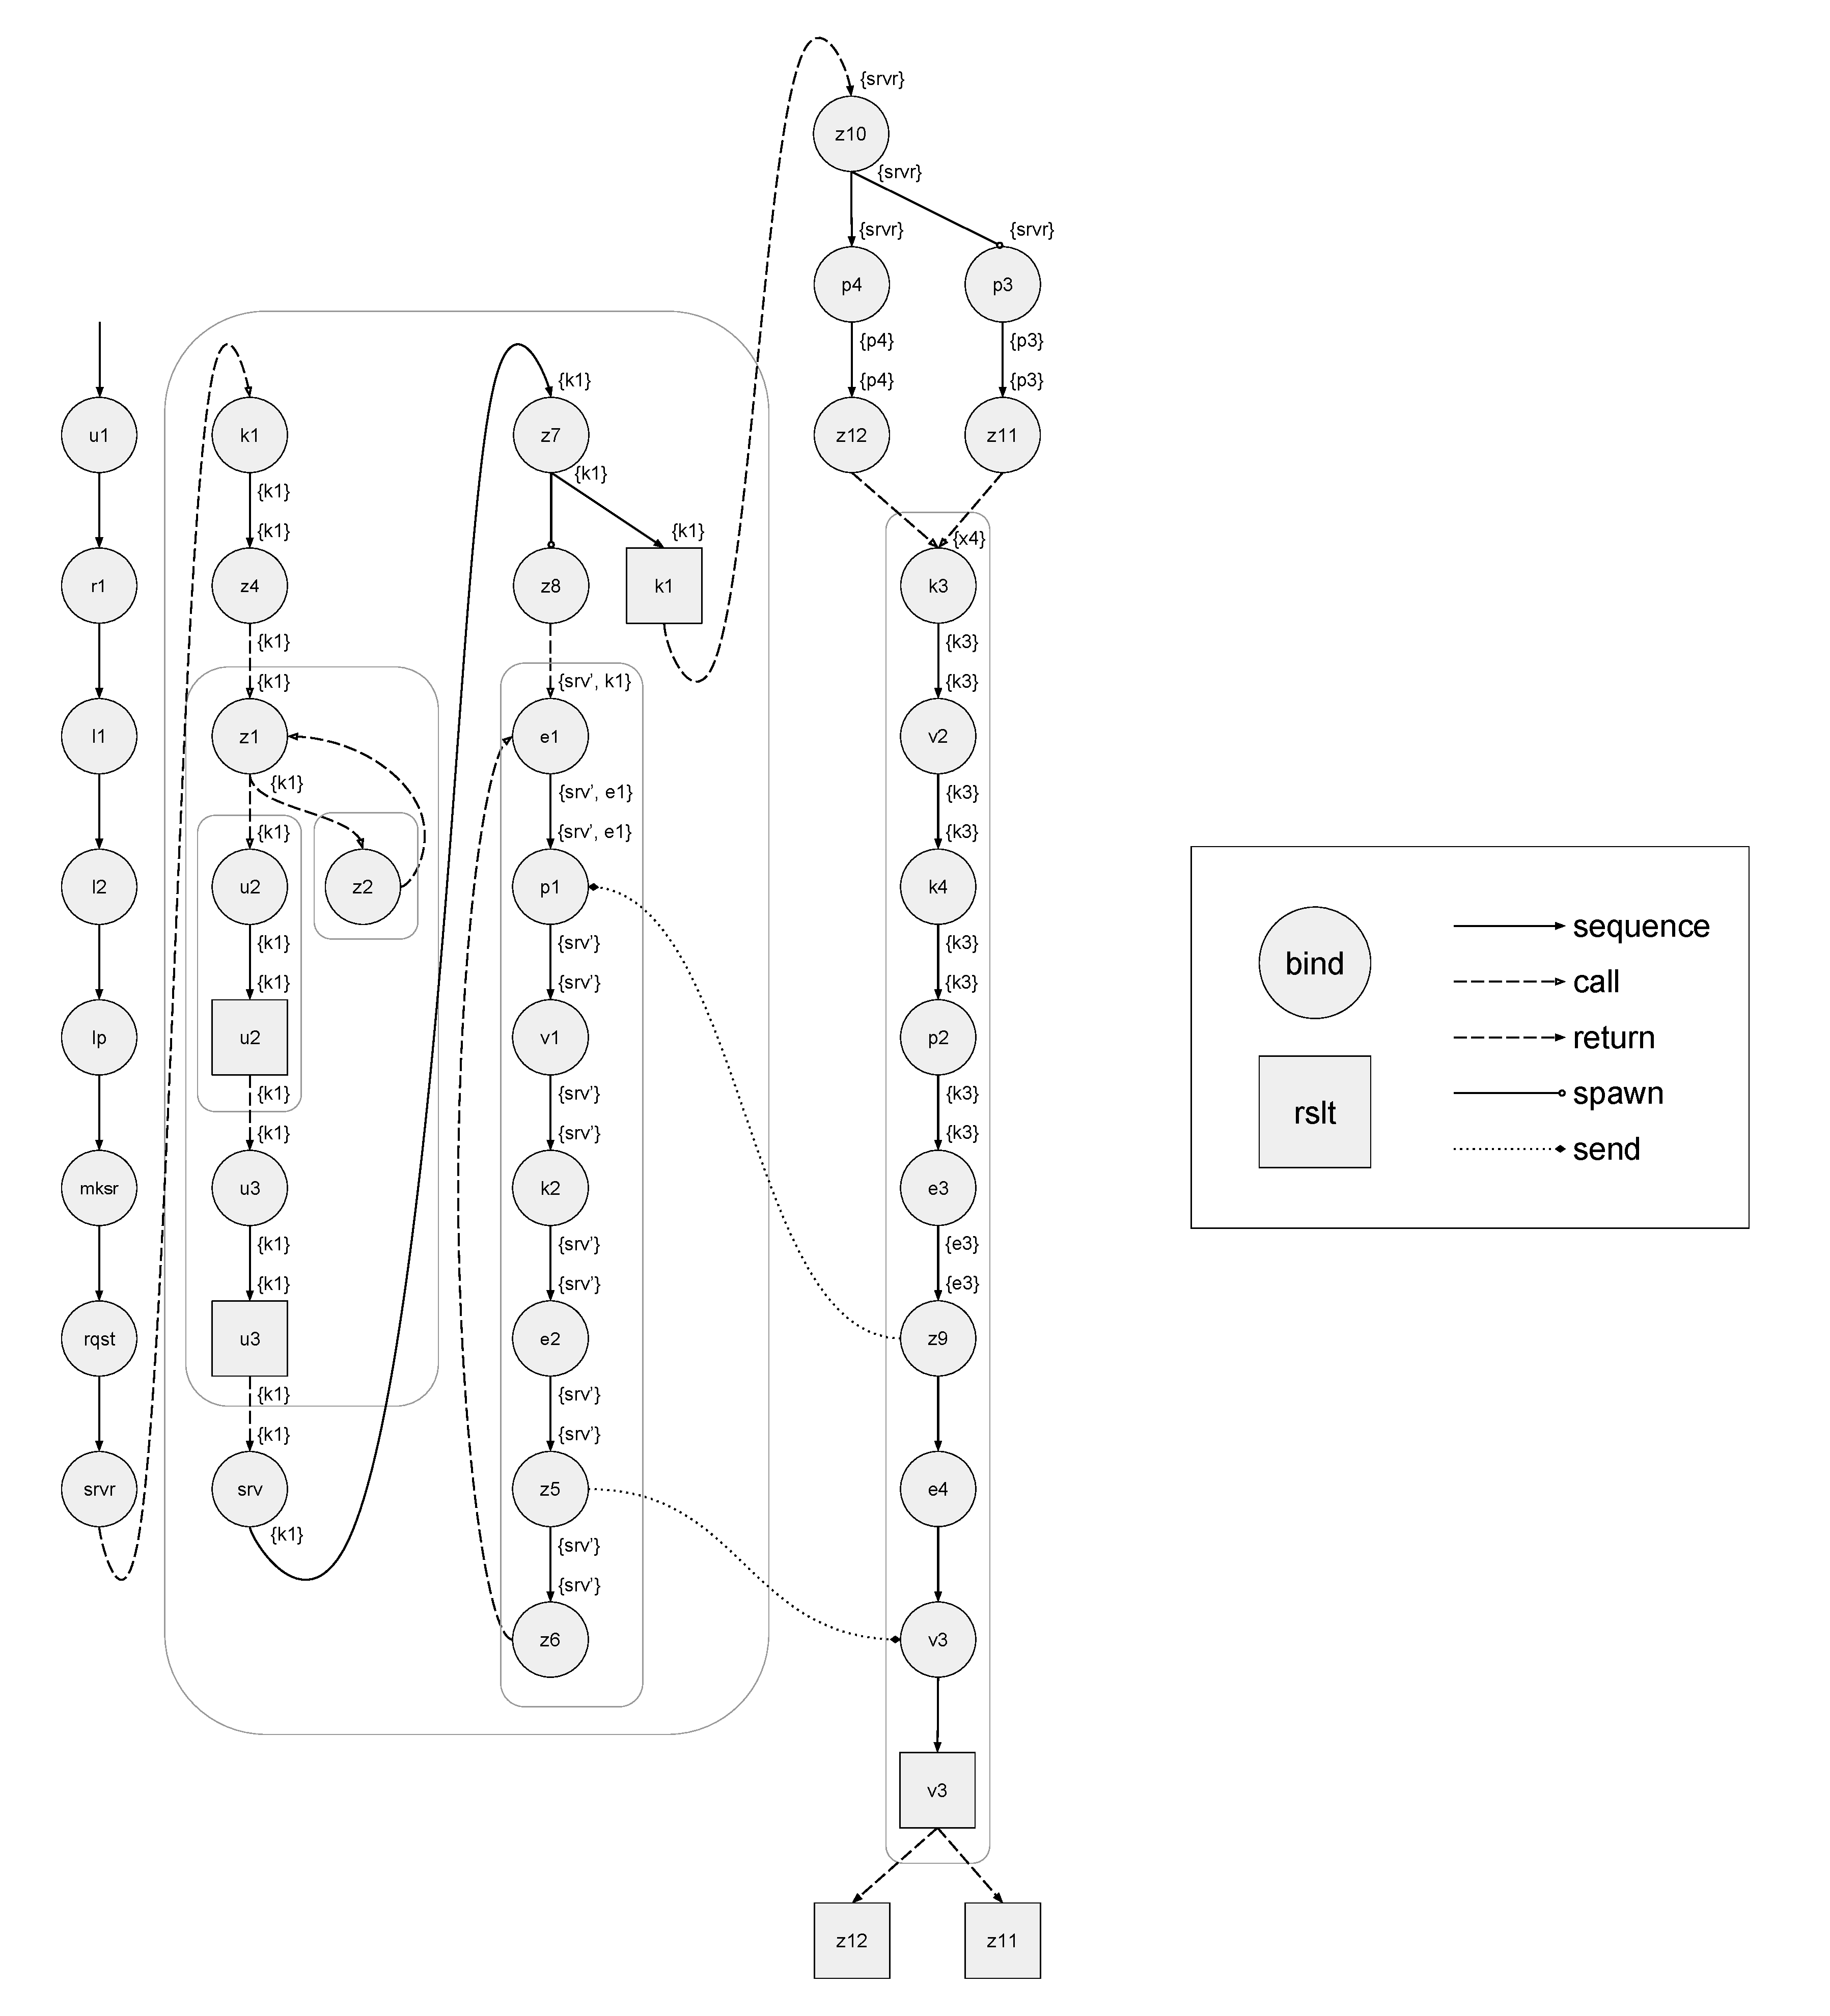
\includegraphics[width=.7\textwidth]{cml-liveness-analysis-k1.pdf}
\end{frame}

\begin{frame}
\frametitle{Higher Precision Analysis}
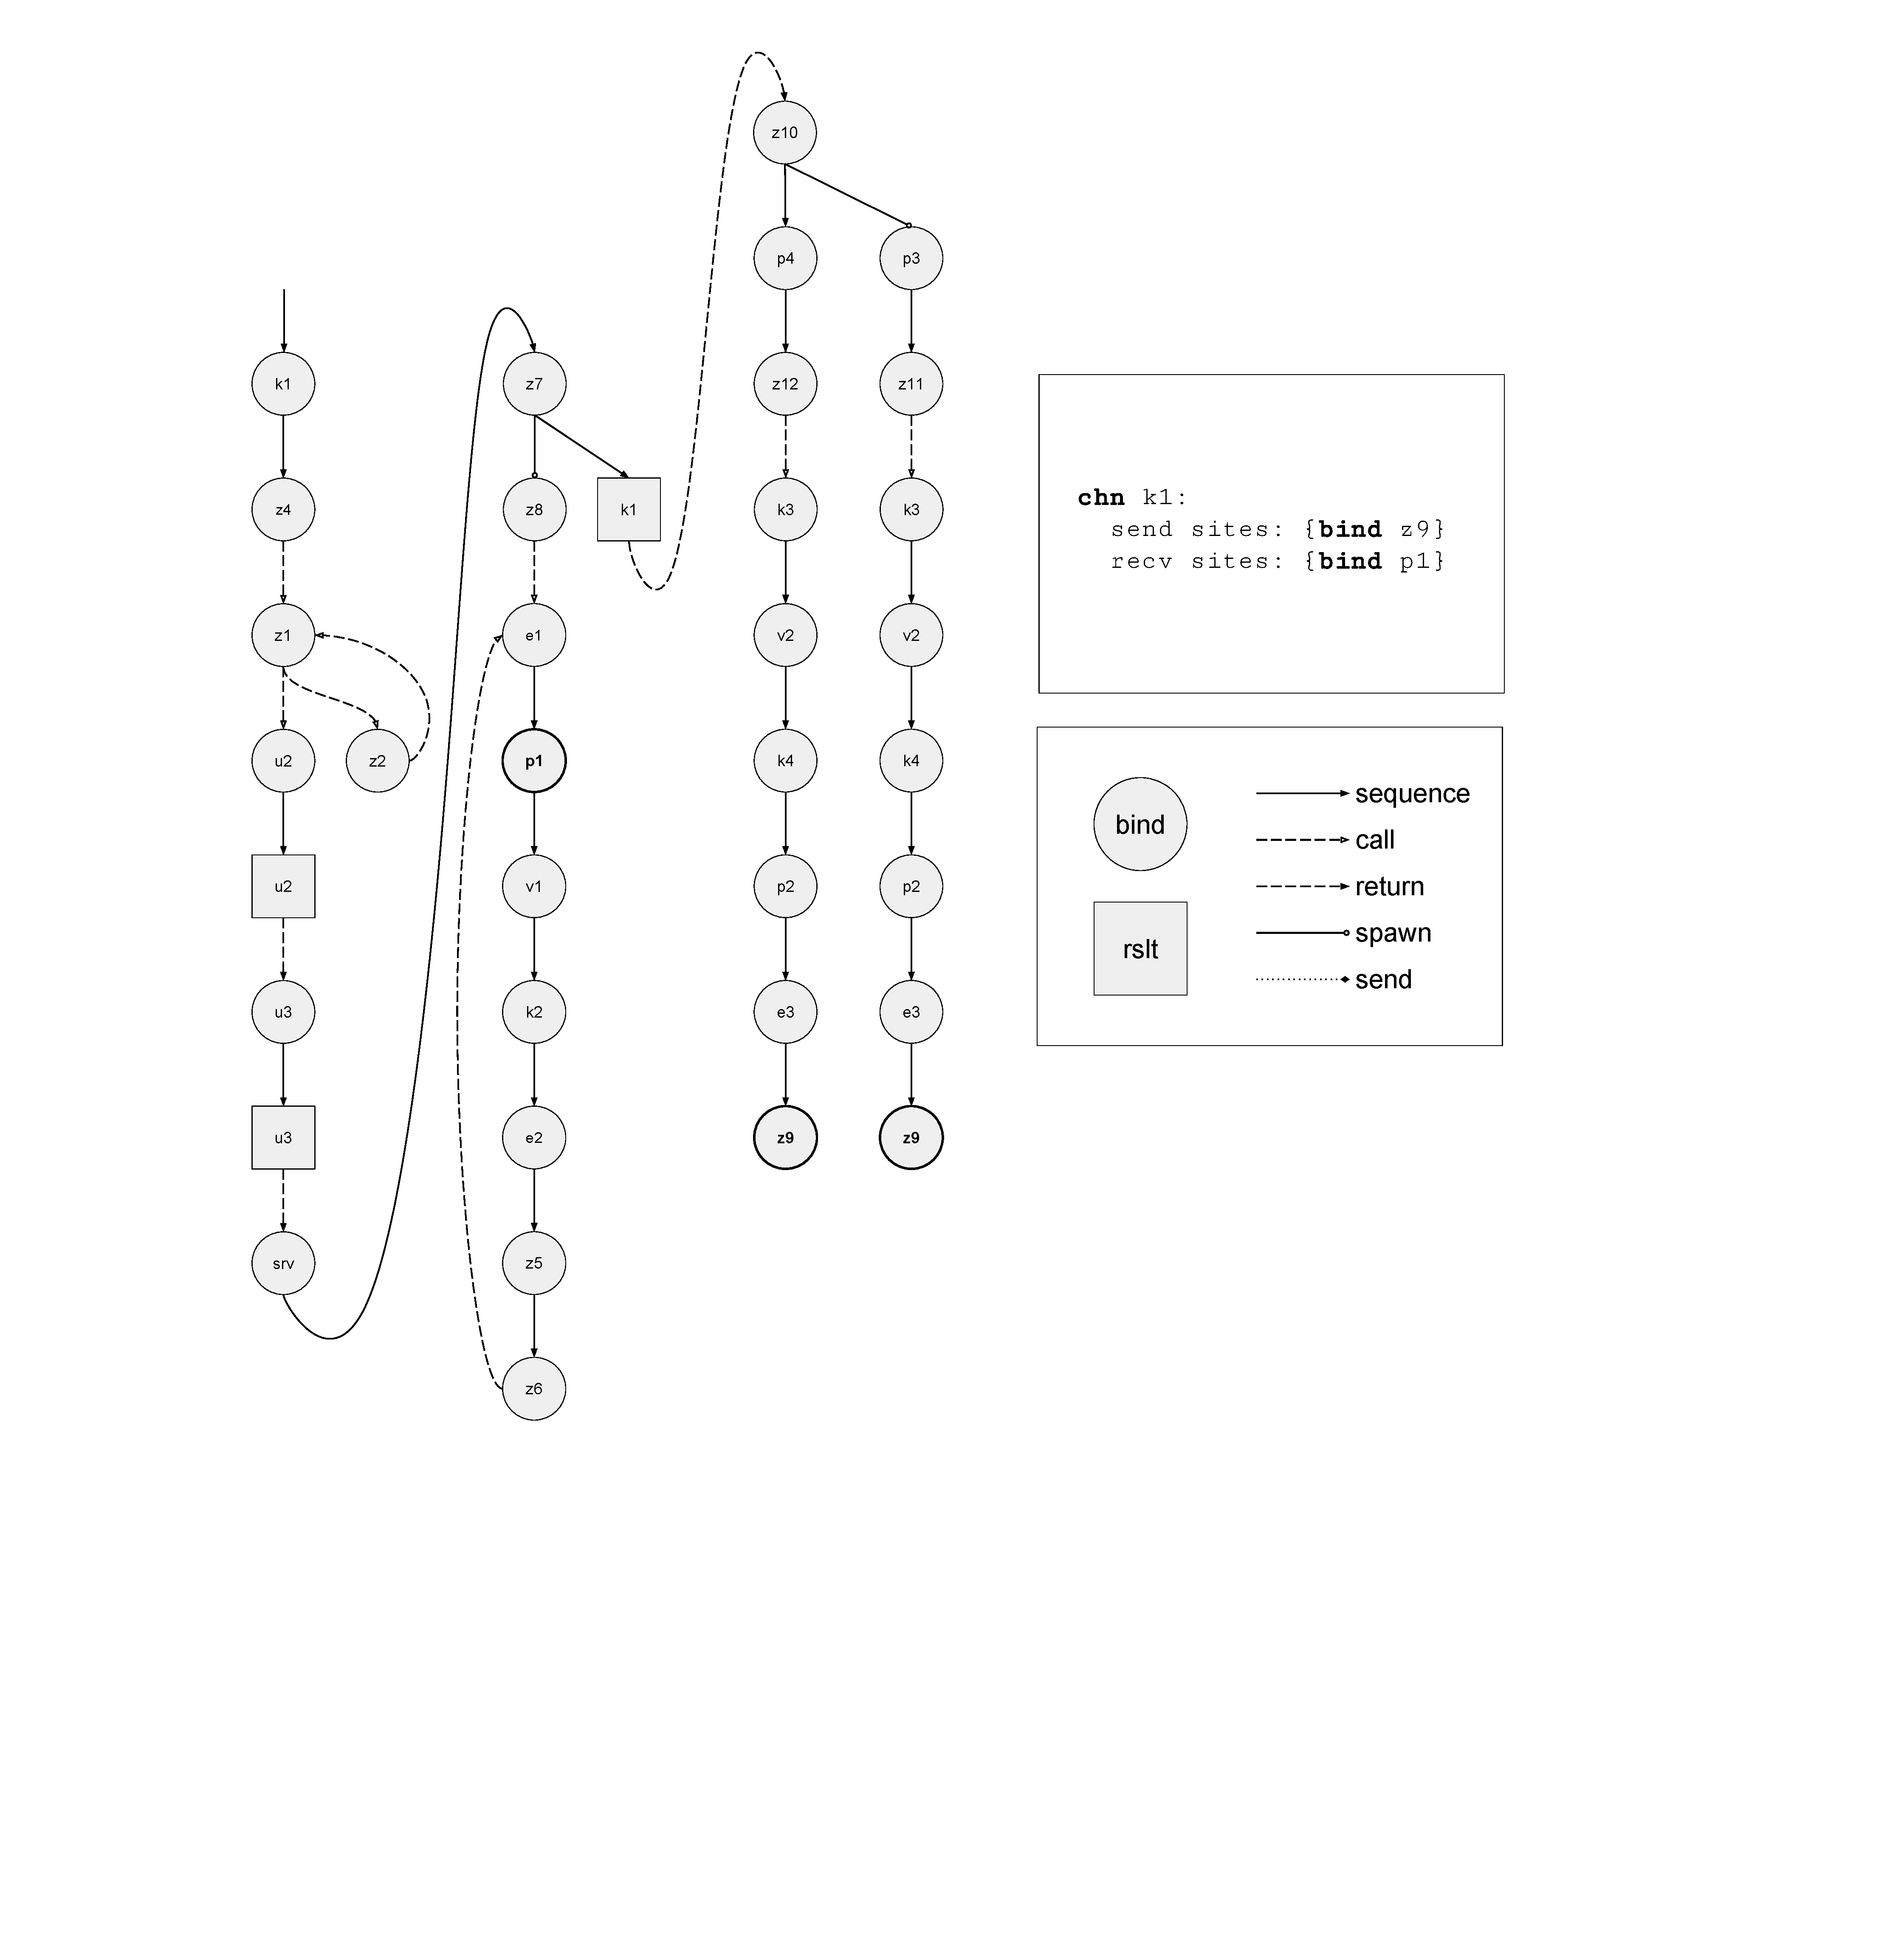
\includegraphics[width=0.7\textwidth]{cml-graph-k1.pdf}
\end{frame}

\begin{frame}
\frametitle{Higher Precision Analysis}
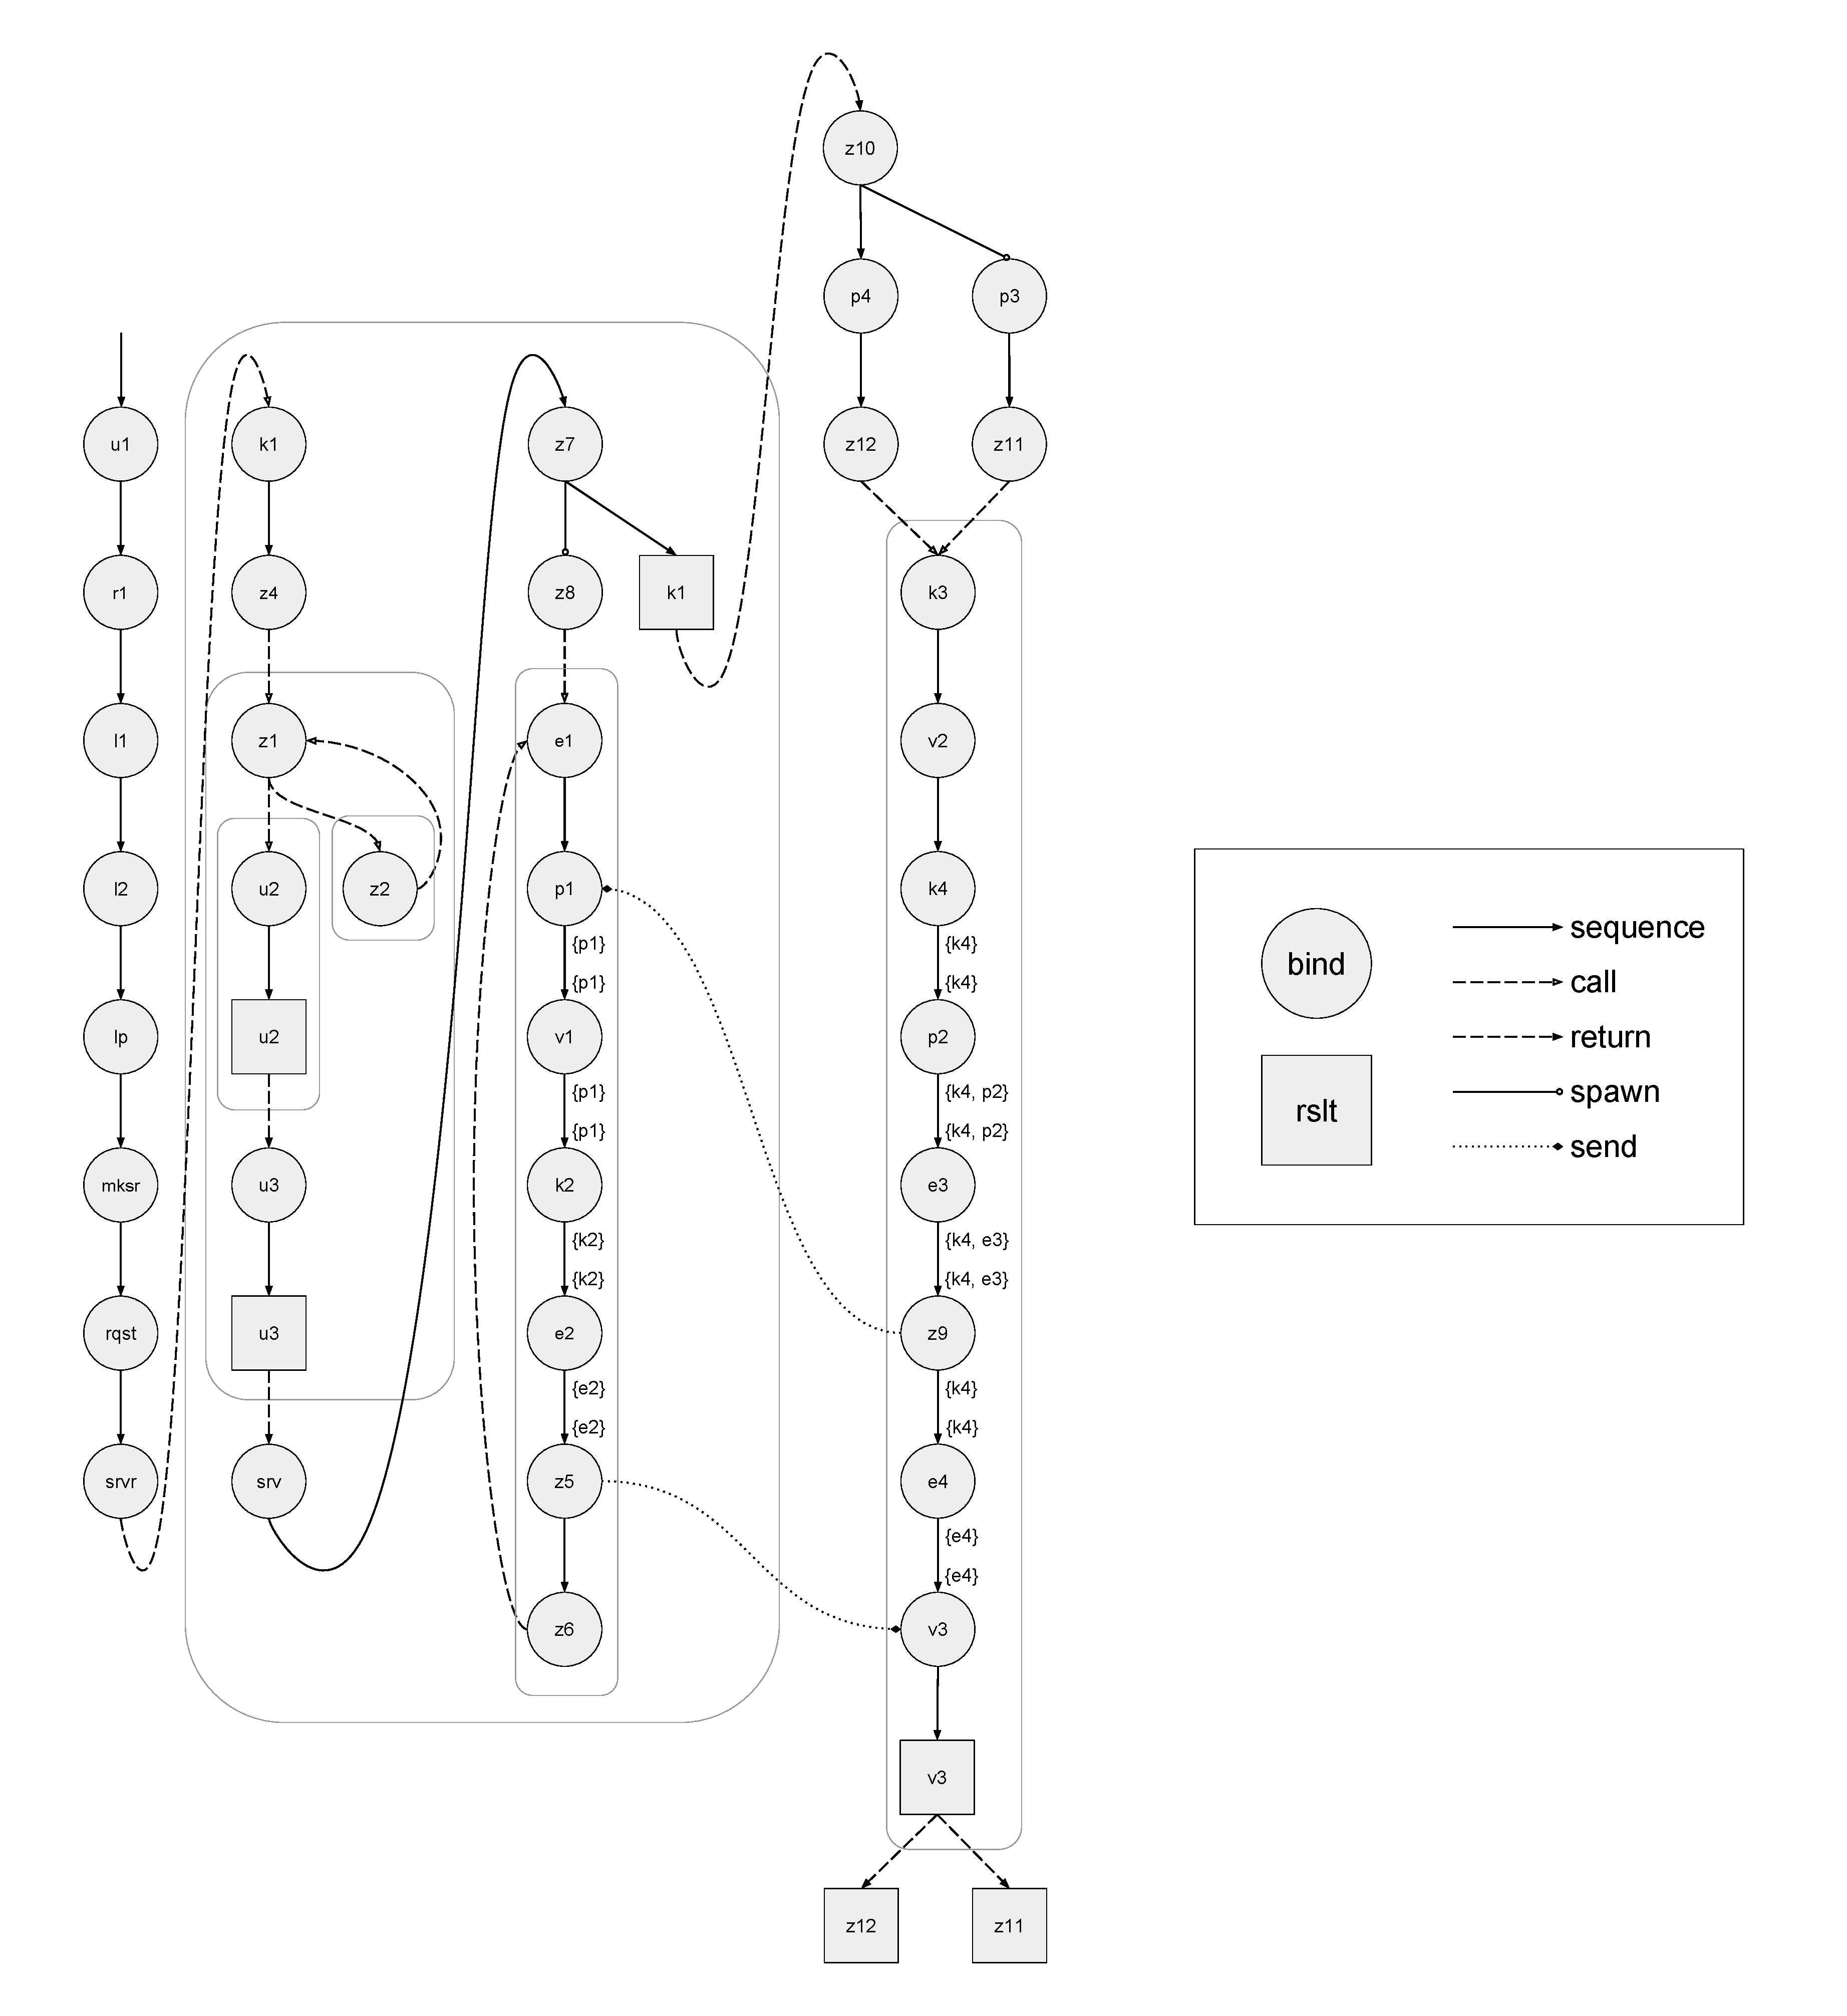
\includegraphics[width=.72\textwidth]{cml-liveness-analysis-k4.pdf}
\end{frame}

\begin{frame}
\frametitle{Higher Precision Analysis}
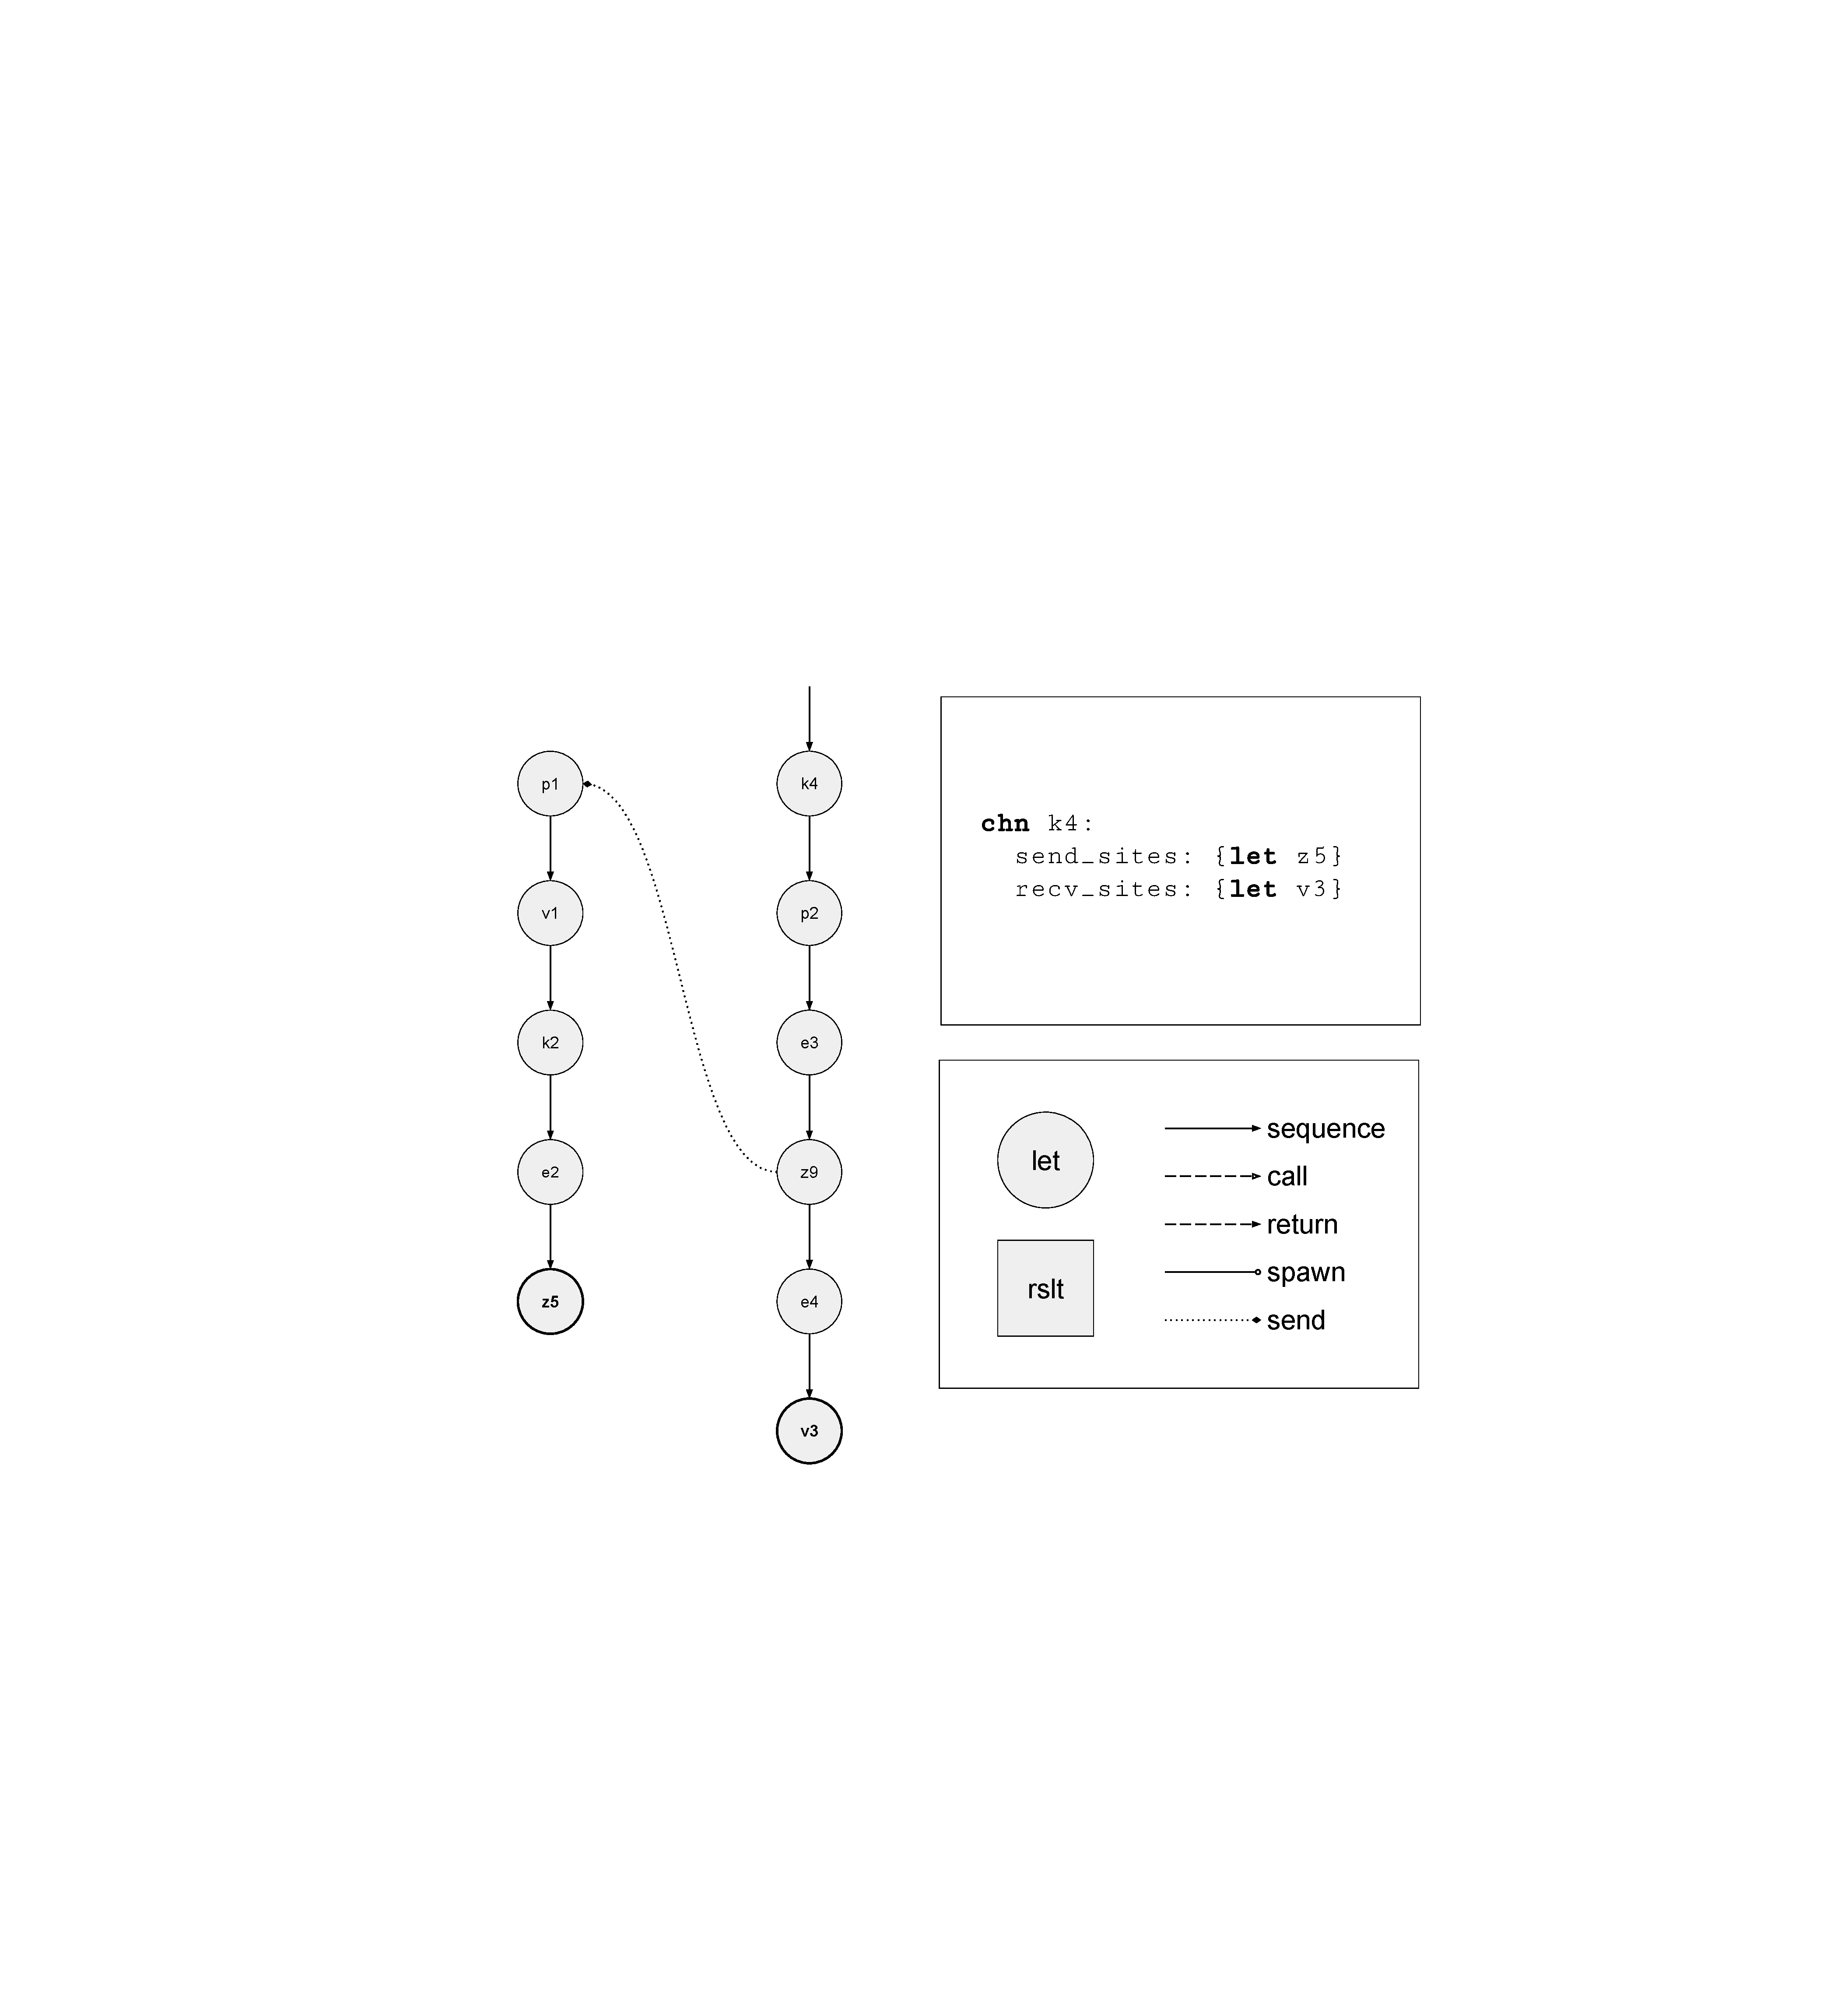
\includegraphics[width=0.6\textwidth]{cml-graph-k4.pdf}
\end{frame}


\begin{frame}[fragile]
\frametitle{Higher Precision Analysis}
\begin{lstlisting}[language=logic, mathescape]
predicate staticOneToMany: term -> name -> bool where
  intro: staticEnv staticComm t graph entr exit n$_c$ 
    staticEval staticEnv staticComm t,
    staticFlowsAccept staticEnv graph t,
    staticChanLive staticEnv entr exit n$_c$ t, 
    forEveryTwo (staticPathLive graph entr exit (IdBind n$_c$)
      (staticSendId staticEnv t n$_c$)) uncompetitive
  $\vdash$ staticOneToMany t n$_c$
\end{lstlisting}
\end{frame}

\begin{frame}[fragile]
\frametitle{Summary}
\begin{itemize}
\item analysis of a simple subset of Concurrent ML
\item formal specification: evaluation, communication classifcation, channel liveness
\item mechanized soundness proofs: evaluation, communication classifcation 
\item formal reasoning techniques: generalization, induction skewing, inference direction 
\end{itemize}
\end{frame}

\end{document}
